\section{병렬화 운영체제 역사}
%20년의 프로세서들은 단일프로세서(uniprocessor) 디자인을 가졌고, 병렬처리와 락은 필요가 없었다. 
%Goal of an OS interface
%Make application developer's job easy
%Allow sharing
%File system, buffer cache, load balancing, etc.
%But, perfectly scalable Efficient implementation

%Three types of parallelism in operating systems
%1. User parallelism
%Users working concurrently with computer
%2. I/O concurrency
%Overlap computation with I/O to keep a processor busy
%3. Multiprocessors parallelism
%Exploit several processors to speedup tasks
%The first two may involve only 1 processor

%This talk: 4 phases in OS parallelism
%Time sharing
%Client/server
%SMPs
%Multicore 60s/70s
%80s/90s
%90s/2000s
%2005s-now Introduction of many ideas for parallelism
%I/O concurrency inside servers
%Multiprocessor kernels and servers
%All software parallel

%POSIX is just the wrong interface
%Shared data fundamentally limits scalability
%Kernels are too big/complex to fix
%Designs cannot keep up with core count

본 장에서는 현시점에서 운영체제 병렬화가 필요한 이유와 함께 운영체제의 병렬화의 역사에 관해서 설명한다.
그동안 운영체제의 병렬화는 시분활 시스템, 클라이언트(client) 서버(server) 구조, 그리고 SMPs(Shared Memory
Processor) 그리고 최근 프로세서에 코어가 많아 지는 멀티코어로 총 4단계에 거처 발전해 왔다~\cite{Kaashoek2015PCO}.

첫 번째 단계에서는 시분활 시스템에서 사용되는 병렬화이다. 
60년대 부터 70년대에서의 운영체제 병렬성은 시분할(time sharing) 시스템을 가졌다.
즉 컴퓨터 한대에 여러 사용자가 동시에 사용되었고, 대부분이 1개의 프로세서로 이루어졌다.
이 시점에서 병렬 처리 연구는 I/O 병렬화 프로그램에 대한 연구가 진행되었다~\cite{Bloch1959EDS}[CTSS 1962]. 
최대한 프로세서를 이용률(utilization)를 높여서 I/O를 처리하기 위해 즉 커널은
 병렬로 I/O를 처리하기 위해 다른 프로그램 커널로 문맥교환되어 실행되도록 만들었다.
 
%Example: the THE operating system [EWD123 1965, SOSP 1967]
%~\cite{Dijkstra1965CSP}
%Technische Hogeschool Eindhoven (THE)
%OS organized as many “sequential” processes
%I A driver is a sequential process
%The THE solution: semaphores

초기 컴퓨터 중 일부 프로세서들은 시분활 시스템과 멀티프로세서의 병렬화를 고려하여
 만들었다(예를 들어, 버로우스(Burroughs)의 B5000~\cite{Mayer1982ABB}).
따라서, 병렬화에 대해서 많은 관심과 노력이 이루어졌다.
그 결과 병렬화 관련 초기 많은 이론인 암달의 법칙~\cite{Amdahl1967VSP}, 멀틱스(Multics)에서의 트래픽 컨트롤
~\cite{Saltzer1966TCM}, 데드락 발견(deadlock detection) 그리고 락 오더링(locking ordering)등
많은 이론들이 생겨나게 되었다. 
70년대 하나의 프로세서 위에서 병렬화를 제공하기 위해 많은 연구 및 개발이 이루어졌고, 실제 
단일 프로세스에 여러 유저에게 시분활 기능으로
 병렬화를 제공하는 Unix 커널~\cite{Ritchie1973UTS}이 개발되었다.

두번째 단계에서는 80년대와 90년대에는 컴퓨터의 가격이 개인이 구매가 가능할 정도 내려갔으며,
 로컬 네트워크로 여러 유저가 
협업하면서 작업할 수 있는 환경이 되어 클라인트 서버 환경을 위한 병렬화가 이루어졌다.
문제는 여러 유저가 수행할 서비스(services)에 대한 병렬화가 필요하게 되었고, 
따라서 논커널 프로그래머들도 커널의 기능이 필요하여, 서버의 커널이 인터페이스(interface)를
 추가하여 유저들에게 병렬화 서비스를 제공하였다. 
 
그 결과 많은 운영체제 병렬화 기술들이 이 시점에 연구 개발되었다. 
예를 들어 스레드(Thread), 락(Locks) 그리고 컨디션 변수(Condition variables)등 이 시점에 많은 연구가 
이루어졌다.
이벤트(events)와 스레드(threads)에 대한 논쟁~\cite{Ous96}~\cite{vonBehren2003WEB}
그리고 Accent~\cite{Rashid1981ACO},
Mach~\cite{Accetta86mach} , V~\cite{Cheriton1983DVK} 등 새로운 운영체제들이 제안되었다. 
이러한 연구들은 마이크로커널(microkernel)에 영감을 주었고, 결국 최근 많은 운영체제가 사용하고 있는 
Pthreads[POSIX.1c, Threads extensions (IEEE Std 1003.1c-1995)]에 대해 영향을 주었다. 
새로운 운영체제 뿐만 아니라 새로운 언어들(예를들어 Mesa~\cite{Lampson1979EPM})도
 연구되었고, 결국 가비지 컬렉션등에 대한 연구가 같이 진행되어, 그 결과 것들이 최근 자바(JAVA)와 고(Go) 언어등에
 영감을 주었다.
결론으로 커널의 인터페이스를 서버 개발자에게 노출하여 서버를 병렬로 이용 할 수 있게 만들었다.

다음 단계에서는 90년대 각각의 프로세서가 메모리를 공유하는 개념의 컴퓨터인 SMP(Shared-memory Multi
Pocessors)가 낮은 가격으로 보급이 되어서, 커널 또는 서버 개발자는 이 떄부터 심각하게 운영체제 병렬화에 대해서 고려하게 되었다.
예를 들어, 운영체제 커널은 BKL(Big Kernel Lock) 등을 지원하며 병렬화 기능을 제공하기 시작하였다.
이 시점 많은 회사(BBN Butterfly, Sequent, SGI, Sun, Thinking Machines 등)가 운영체제 병렬화에 대해서 
연구하기 시작했다.
그 결과 많은 운영체제 성능 확장성에 대해서 새로운 개념 예를들어, 
MCS 락~\cite{MellorCrummey1991MCS}, 유저 레벨 쓰레딩~\cite{Marsh1991FUT},
 NUMA 메모리 관리~\cite{Bolosky1991NPR}, 가상 머신 모니터(virtual machines monitor)
~\cite{Bugnion1997DRC} 등이 제안되었다.  


\begin{figure}[h]
  \begin{center}
    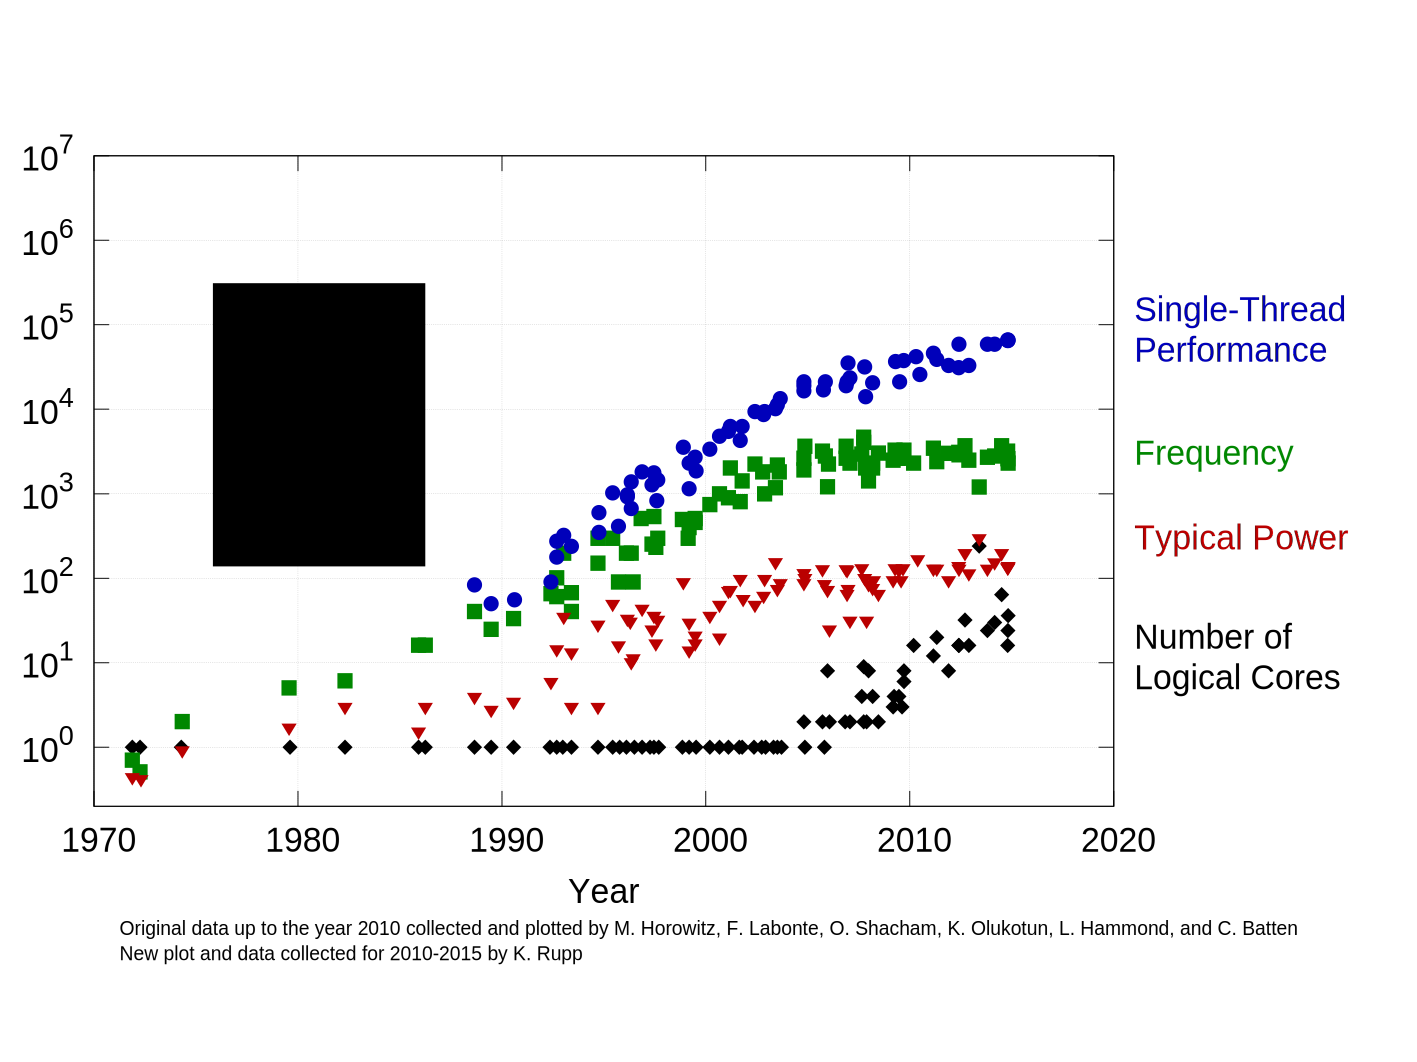
\includegraphics[scale=0.3]{fig/cpu}
  \end{center}
  \caption{CPU 발전 동향.}
  \label{fig:aim7}
\end{figure}

마지막 단계는 멀티코어이다.
그림 ~\ref{fig:aim7}과 같이 주파수는 계속 증가하다가, 2000년대 중반 멈추고, 그
때부터 코어수가 증가하고 있다. 
따라서 코어수가 100개 이상의 멀티코어 프로세서들도 등장함에 따라, 공유 때문에 야기하는 
새로운 문제가 발생하기 시작하였다. 
최근에 발생하는 문제들은 상당 부분이 캐시라인(cache-line)의 공유 때문에 발생하는 문제이고, 
이를 해결하기 위해서 최근에는 여러 운영체제(section~\ref{sec:osrelated}),
 락 기법(section~\ref{sec:lockrelated}), 그리고 자료구조와
 알고리즘(section~\ref{sec:datarelated})들이 개발되고 있다.

%$$$$$$$$$$$$$$$$$$$$$$$$$$$$$$$$$$$$$$$$$$$$$$$$$$$$$$$$$$$$$$$$$$$$$$$$$$$$$$$$
%Paragraph 1:Linux Scalability의 연구에 대한 설명
%$$$$$$$$$$$$$$$$$$$$$$$$$$$$$$$$$$$$$$$$$$$$$$$$$$$$$$$$$$$$$$$$$$$$$$$$$$$$$$$$

\newpage
\section{최근 운영체제 병렬화 연구}
\label{sec:osrelated}

%To improve the scalability, researchers have attempted to create new
%operating systems~\cite{Boyd-WickizerCorey}~\cite{Wentzlaff2010fOS}
%~\cite{Baumann2009Barrelfish}~\cite{Zellweger2014Multikernel}
%~\cite{Liu2009Tessellation}~\cite{Farrington2010Helios}
%or have
% attempted to optimize existing operating
%
 % systems~\cite{SilasBoydWickizer2010LinuxScales48}~\cite{AustinTClements2012RCUBalancedTrees}~\cite{Clements2013RadixVM}~\cite{SilasBoydWickizerPth} ~\cite{Changwoo2016UMSF}.
 
코어 수가 증가되는 상황에서 병렬화가 중요해진 운영체제에 대한 연구는 성능에
 대한 확장성을 향상시키기 위해서, 새로운 확장성 있는
운영 체제를 만들거나 ~\cite{Boyd-WickizerCorey}~\cite{Wentzlaff2010fOS}
~\cite{Baumann2009Barrelfish}~\cite{Zellweger2014Multikernel}
~\cite{Liu2009Tessellation}~\cite{Farrington2010Helios} 
기존 운영체제를 최적화 시키는
방법~\cite{SilasBoydWickizer2010LinuxScales48}
~\cite{AustinTClements2012RCUBalancedTrees}~\cite{Clements2013RadixVM}~\cite{SilasBoydWickizerPth}을
시도하고 있다.
%Our research belongs to optimizing existing operating systems in order to
%solve the Linux fork scalability problem.
%이 중 우리의 연구는 리눅스의 fork에 대한 확장성을 개선하기 위한
% 기존 운영체제를 최적화 하는 방법에 속한다. 
%However, previous research did not deal with the anonymous reverse mapping,
%which is one of the fork scalability bottleneck.
%하지만 기존 연구들은 fork의 확장성 병목 지점 중 하나인 익명 역 매핑에 대해서는 처리하지 않았다.

%Cache-line fetches are expensive
%Read cache line written by
%another core: expensive!
%100–10000 cycles
%(contention)

%For reference, a creat system call costs 2.5K cycles
%Avoiding cache-line sharing is challenging
%Consider read-write lock
%struct readwritelock {
%int count;
%// -1, write mode; > 0, read mode
%listhead waiters;
%%spinlock waitlock;
%}
%Problem: to acquire lock in read mode requires modifying count
%%Fetching a remote cache line is expensive
%Many readers can cause performance collapse

\subsection{Corey}

Corey는 MIT의 Parallel and Distributed Operating Systems Group에서 개발하였다. 
기본적인 철학은 커널 영역의 공유 데이터를 유저 응용프로그램이 사용할 수 있게 만들어 주어서, 
공유 데이터 때문에 발생하는 경합 문제를 유저에게 해결할 수 있도록 제공하는 것이다. 
따라서 유저 응용프로그램의 워크로드에 따라 경유 문제를 해결할 수 있는 방향을 제공해준다.
이것은 exokernel[]의 개념을 가져와서 매니코어 시스템에 적용하였고, 이를 통해 성능 확장성을 개선하였다.

이러한 Corey는 3가지 기본적은 개념을 가지고 있다. 그것은 공유(shares), 주소 트리(address trees)과 커널
코어(kernel core)이다.
공유는 어떻게 커널 자료구조를 접근할 수 있는지에 대해서 제공해준다.


\subsection{Barrelfish}

Barrelfish 운영체제는 취히리의 ETH와 마이크로 소프트(Microsoft)가 공동연구하여 만든 운영체제이다. 
또는 멀티커널(multikernel)이라고도 부른다.
기본적인 철한은 공유 메모리 시스템 기능들을 모두 분산 처리 방식으로 구현하자는 것이다.


\subsection{fOS}

fOS(Factored operating system)은 역시 Massachusetts Instiute of Technoloy에서 개발한
Corey와 비슷한 개념의 운영체제이다. 
fOS의 5가지의 설계 철학을 가지고 있다. 

\subsection{Tessellation}

Tesselation 운영체제는 버클리에서 만든 클라인어트 운영체제이다.
이것이 기본철학은 시간과 공간을 파티션하여 동작시키도록 만든 하나의 파티션닝 운영체제이다.


\subsection{BonsaiVM}

BonaiVM은 MIT Parallel and Distributed Operating Systems Group에서 개발한 리눅스 커널을 위한 
가상 메모리 시스템이다. 
이것은 새로운 운영체제를 제안하는 것이 아니라, 리눅스 커널을 대상으로 개선한 연구이며, 
리눅스 커널 중 가상 메모리 시스템을, RCU라는 동기화 기법을 사용하여 성능 확장성을 향상시킨 연구이다.


\subsection{RadixVM}

RadixVM은 기존 SV6 운영체제에 대해서 가상 메모리에 대한 부분을 성능 확장성 있게 만든 연구이다.
리눅스는 너무 복잡한 구현으로 인하여, 적용하기 힘은 개념을 덜 복잡한 운영체제에 적용하였다. 

\subsection{OpLog}

OpLog는 RCU와 반대로 업데이트 비율이 높은 업데이트 헤비(Update heavy)한 자료구조를 위해 만든 
동기화 기법 중 하나이다.

%BonsaiVM~\cite{AustinTClements2012RCUBalancedTrees} solved this address space
%problem by using the RCU;
%RadixVM~\cite{Clements2013RadixVM} created a new VM using refcache and radix
%tree, which enable \code{munmap}, \code{mmap}, and \code{page fault} on
%non-overlapping memory regions to scale perfectly.
%Alternatively, to avoid contention caused by shared address space locking,
%system programmers change their multithreaded applications to use
%processes~\cite{SilasBoydWickizer2010LinuxScales48}.

%$$$$$$$$$$$$$$$$$$$$$$$$$$$$$$$$$$$$$$$$$$$$$$$$$$$$$$$$$$$$$$$$$$$$$$$$$$$$$$$$
%Paragraph 3: Scalable Data Structure and Lock에 대한 연구
%$$$$$$$$$$$$$$$$$$$$$$$$$$$$$$$$$$$$$$$$$$$$$$$$$$$$$$$$$$$$$$$$$$$$$$$$$$$$$$$$
\newpage
\section{확장성 있는 락 연구}
\label{sec:lockrelated}
%Scalable locks have been designed by the
%queue-based locks~\cite{MellorCrummey1991MCS}~\cite{Magnusson1994QLC},
%~\cite{Wang2016BeMyGuest},
%~\cite{Scott2013SS}
%~\cite{Bueso2014MCS}~\cite{Bueso2015STP}
%hierarchical locks~\cite{Radovic2003HBL}~\cite{Chabbi2016CLL} and
%~\cite{Luchangco2006HCQ}
%~\cite{Chabbi2015HPL}
%delegation
% techniques~\cite{Hendler2010FC}~\cite{Fatourou2012RCS}~\cite{Delegation2014}.

%Scalable locks have been designed by the
%queue-based locks~\cite{MellorCrummey1991MCS}~\cite{Magnusson1994QLC},
%~\cite{Wang2016BeMyGuest},
%~\cite{Scott2013SS}
%~\cite{Bueso2014MCS}~\cite{Bueso2015STP}
%hierarchical locks~\cite{Radovic2003HBL}~\cite{Chabbi2016CLL} and
%~\cite{Luchangco2006HCQ}
%~\cite{Chabbi2015HPL}
% delegation
%techniques~\cite{Hendler2010FC}~\cite{Fatourou2012RCS}~\cite{Delegation2014}.
확장성 있는 락들은 큐 기반의 락~\cite{MellorCrummey1991MCS}~\cite{Magnusson1994QLC},
~\cite{Wang2016BeMyGuest},
~\cite{Scott2013SS}
~\cite{Bueso2014MCS}~\cite{Bueso2015STP}과 계층적 락~\cite{Radovic2003HBL}~\cite{Chabbi2016CLL} and
~\cite{Luchangco2006HCQ}
~\cite{Chabbi2015HPL} 그리고 위임하는 방법(delegation
techniques)~\cite{Hendler2010FC}~\cite{Fatourou2012RCS}~\cite{Delegation2014}을 사용한다.
%Some approaches have been gradually adapted in real production software.
%For example, Linux kernel has replaced non-scalable locks with
%MCS locks~\cite{overviewofkernellock}.
%Our research is similar to the delegation techniques because
%the \LDU's \code{synchronize} function runs as a
%combiner thread;it improves cache locality.
이 중 우리의 연구는 LDU의 \code{synchronize} 함수가 마치 FC의 컴파이너 쓰레드(combiner thread)와 같이
동작함으로 위임하는 방법과 비슷하다. 이것은 캐시의 지역성을 높이는 방법이다.
%However, our approach not only can improve cache locality but also
%can eliminate synchronization methods during updates due to using a lock-free
% manner.
하지만, 우리의 방법은 캐시의 지역성을 높일 뿐만아니라 업데이트 명령을
 수행하는 동안 락 프리(lock-free) 방법으로 동기화 기법들을 제거 할 수 있다. 
%MCS~\cite{MellorCrummey91}, a scalable lock.
%, is used in the Linux
%.
%In read-mostly data structures, RCU~\cite{McKenney98} can be quite useful.
%However, 


%\subsection{Ticket Lock}



%티켓 락은 (Ticket Lock)은 

%\subsection{Queued Lock - 수정}



%\subsection{Delegation techniques}

%Flat Combining은 




%$$$$$$$$$$$$$$$$$$$$$$$$$$$$$$$$$$$$$$$$$$$$$$$$$$$$$$$$$$$$$$$$$$$$$$$$$$$$$$$$
%Paragraph 2:Concurrent updates에 대한 연구
%$$$$$$$$$$$$$$$$$$$$$$$$$$$$$$$$$$$$$$$$$$$$$$$$$$$$$$$$$$$$$$$$$$$$$$$$$$$$$$$$
\newpage
\section{확장성 있는 자료구조 연구}
\label{sec:datarelated}
%Many scalable data structures with scalable schemes show different performances
% depending on their update ratios.
많은 확장성 있는 방법과 사용되는 자료구조들은 업데이트 비율에 따라 다른 성능을 가진다.  
%In low and middle update rate, researchers have attempted to create new
% scalable schemes~\cite{McKenney98}~\cite{Matveev2015RLU}~\cite{Harris2001Lockfree}
%~\cite{Fomitchev2004Lockfree}
%~\cite{Timnat2012}
%or have attempted to adapt these scheme to data
%structures~\cite{Arbel2014ConcurrentRCU}~\cite{Dodds2015SCT}~\cite{AustinTClements2012RCUBalancedTrees}.
낮거나 중간 정도의 업데이트 비율에서는 연구자들은 새로운 확장성있는
기법~\cite{McKenney98}~\cite{Matveev2015RLU}~\cite{Harris2001Lockfree} ~\cite{Fomitchev2004Lockfree}
~\cite{Timnat2012}을 연구하거나 그 기법을 자료구조에 
적용~\cite{Arbel2014ConcurrentRCU}~\cite{Dodds2015SCT}~\cite{AustinTClements2012RCUBalancedTrees}을
하도록 시도하고 있다.
%In high update rate, the OpLog shows significant improvement in
%performance scalability for update-heavy data structures in
%many core systems, but suffers from limitation and overhead due
%to time-stamp counter management.
높은 업데이트 비율에서는 OpLog가 매니코어의 업데이트 비율이 높은 자료 구조에 대해서
 상당히 높은 성능 확장성을 가진다. 
%We substantially extend our preliminary work~\cite{Kyong2016LDU} not only to
% support per-core algorithm but also to apply the \LDU to anonymous rmap due to improving the
%Linux kernel scalability.


%\subsection{RCU}

%RCU는 \ldots
%Read-copy update (RCU) becomes popular
%Readers read shared data without holding any lock
%Mark enter/exit read section in per-core data structure
%Writer makes changes available to readers using an atomic
%instruction
%Free node when all readers have left read section
%Lots of struggling to scale software.

%\subsection{Non-blocking Algorithms}

%Non-blocking 알고리즘은\ldots

%\subsection{RLU}

%RLU는 \ldots


%\newpage
%\section{하드웨어}
%\label{sec:hwrelated}

%\subsection{캐시 일관성(Cache Coherency)}

%병렬화를 위한 캐시는\ldots 

%\subsection{원자적 명령(Atomic Operations)}

%원자적 명령은\ldots

%\subsection{메모리 배리어(Memory Barriers)}

%메모리 배리어는\ldots

